\subsection{FSR Mathematik}
\label{page:fsr}
Unsere Aufgabe ist es, die Interessen der Fachschaft -- das seid ihr und alle
anderen Mathematik-Studenten am Fachbereich Mathematik der Universität Hamburg --
zu vertreten. Wir werden zu Beginn jedes Semesters auf einer Vollversammlung
aller Mathematik-Studenten gewählt und kümmern uns dann um alles, was so anliegt.

Konkret bedeutet das: Wir beobachten, was hier am Fachbereich, in der Fakultät,
an der Uni und sonst wo vor sich geht und mischen uns wenn nötig ein und
informieren euch über alles Wichtige durch unseren E-Mail-Newsletter (hierfür
nutzen wir die Mailinglisten des Fachbereichs -- also ganz schnell eintragen!)
und Aushänge in unserem Infokasten (zwischen den Fahrstühlen und der
Pförtnerloge neben dem schwarzen Brett) oder der Pinnwand neben
dem T30. Bei wichtigen Anlässen berufen wir auch während des Semesters
Vollversammlungen (VV) ein, auf denen wir mit euch das weitere Vorgehen
besprechen. Dies geschah in der Vergangenheit vor allem zu Streiks oder
Aktionen gegen Studiengebühren.

Darüber hinaus sind wir eure Ansprechpartner für Probleme mit eurem Studium und
für Fragen aller Art. Wir wissen zwar auch nicht auf alles eine Antwort, aber
haben dann meistens eine Idee, wer euch weiterhelfen kann.

Wir unterhalten auch eine Sammlung von Prüfungsprotokollen, die euch zur
Vorbereitung auf eure eigenen Prüfungen sicher hilfreich sein kann. Diese lebt
von der Mithilfe aller, das heißt wer eine Prüfung absolviert hat, sollte im
Anschluss ein simples Gedächtnisprotokoll verfassen und über die Datenbank auch
anderen zur Verfügung stellen. So bleibt die Sammlung stets möglichst aktuell,
und alle haben einen Nutzen davon. Gerade über die Prüfungen in den
Bachelorstudiengängen gibt es natürlich noch kaum Protokolle, also wäre es sehr
hilfreich Kopien der Klausuren zu bekommen.

Ansonsten veranstalten wir als FSR auch noch diverse Aktionen für euch, wie zum
Beispiel jeweils ein Skat- und Pokerturnier, öfters mal
Überraschungswunschfilmabende, jährliche Weihnachtsfeiern, seltener
Spieleabende sowie ab und zu Partys oder ein Sommergrillen und was uns gerade
sonst noch so einfällt -- oder von euch gewünscht wird. Falls ihr eine Idee
oder eine Wunsch habt, was veranstaltet werden könnte, meldet Euch einfach bei
uns!

Im Semester gibt es meistens feste Sprechzeiten, während der ihr auf jeden Fall
einen von uns im T30 antreffen solltet. Ansonsten erreicht ihr uns per Mail an
fsr@math.uni-hamburg.de.

\begin{center}
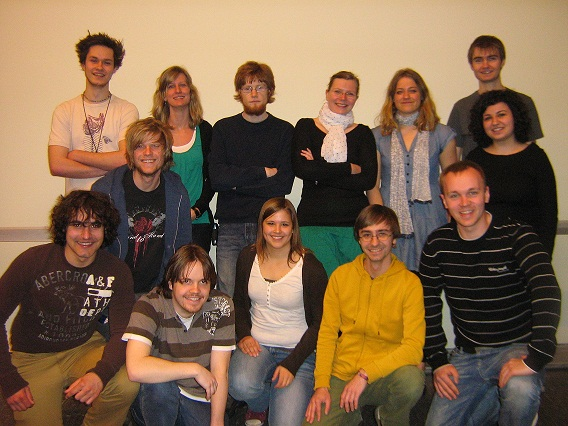
\includegraphics[scale=1.5]{images/fsrsose2011}
\end{center}

Der Fachschaftraum T30 ist übrigens ein studentischer Aufenthaltsraum, der
allen Studenten offen steht. Hier findet ihr neben der Datenbank mit
Prüfungsprotokollen eine kleine Präsenzbibliothek, welche vor allem die gängige
Anfängerliteratur zum schnellen Nachschlagen oder einfach mal so Stöbern
bereithält. Ansonsten liegen dort auch immer mal wieder aktuelle
Informationsmaterialien, die für den einen oder anderen interessant seien können.

Aber auch alles, was man braucht, um sich mal eine kleine Lernpause zu gönnen,
findet ihr im T30. Es gibt Getränke zum Selbstkostenpreis, Geschirr für eure
selbst mitgebrachte Mahlzeit, falls die Mensa schon zu hat (dieses ist nach
Benutzung wieder zu reinigen) und meist auch einige motivierte Mitspieler für
die eine oder andere Doppelkopf, Poker oder Skatrunde oder einfach offene
Ohren, um mal ein wenig Lernfrust abzulassen oder sich einen Lösungstipp zu
holen.

Wer Lust hat, mehr über uns zu erfahren und vielleicht sogar bei uns
mitzuarbeiten, ist herzlich zu einem Besuch im T30 oder auf unserer Homepage
\url{http://www.math.uni-hamburg.de/fsr} eingeladen.

In den nächsten Wochen findet die Wahl des neuen FSR statt. Dabei wird über das
Programm für das Semester diskutiert, also kommt zur Vollversammlung und bringt
eure Wünsche und Vorstellungen ein. Achtet dazu auf Ankündigungen am Infobrett
und auf der Tafel im Foyer.

\hfill euer FSR Mathematik

\hfill Alex, Anna, Arne, Bijan, Dennis, Fabian, Ines, Justus Kathrin, Rike,
Steffen, Svenja, und Tim
